\section{Implications for \pol{}}
\label{sec:implications}

\subsection{Five tensions in the specification}
\label{sec:synthesis}

Read against the evidence, the specification pulls in two directions at five points. Because typed judgement is cheap, an implementation's defaults are likely to settle each of them.
For each tension we give the most charitable reading of the text, the evidence that bears on it, and options, at least one of which preserves the text.
The choice belongs to the framework's authors and its implementers.

\paragraph{T1. Understanding emotion in language versus detecting persons' emotional states.}
\Clause{4.3} states that it is ``entirely unnecessary'' for PAI to detect a person's emotional state, while \clause{4.3.3.1} asks PAI to ``understand human emotional states and processes''.
On one consistent reading, PAI recognises the emotional meaning and intent of utterances and never infers a person's inner state.
The text does not state this boundary, and a typed model makes it almost free to attach an emotion score to every message.
The evidence on emotion-related judgement is thin and mixed~\cite{arx24574,arx35293}, and inferring emotion from observable signals is scientifically weak~\cite{barrett2019emotional}.
\emph{Options:} state the boundary explicitly, and reserve emotion-related judgement for PAI auditing its own outputs, for example for the fabricated intimacy that \clause{4.3.2} names as manipulation.

\paragraph{T2. Binary verdicts versus a three-valued ethics.}
A yes/no question such as ``is this hate language?'' discards both the state of absence (\clause{4.3.2}) and the warning that the concepts are not moral labels (\clause{1.5}).
The evidence points the same way (G3, G4).
Option names can drive the verdict, and where the model is unsure, complementary probabilities do not sum to one.
An explicit ``I don't know'' is rarely chosen when correct, and ``none'' only inconsistently.
\emph{Options:} make every love/hate question three-valued, with absence or insufficient information as an explicit option, and ask sufficiency as its own question.
Keep ``contested'' (people disagree) as a separate flag routed to people, and keep moral vocabulary out of option names by binding neutral identifiers to definitions.
These options implement \clause{1.5} and \clause{4.3.2} as written.

\paragraph{T3. Full transparency versus closed models.}
\Art{4} and \art{5}(4) require that operating logic and decision processes be ``completely open and transparent'' and that technology ``should not be a black box'', but the weights, architecture, reward and training data of hosted \jev{} are unpublished~\cite{arx24574,arx28919}.
Logging a closed component's inputs, outputs, versions and calibration data partly satisfies \art{4} but cannot show how the component reaches its outputs.
Open models make the readout inspectable, but were in several comparisons less accurate or less robust~\cite{arx26758,arx33401}, although the gap is not fixed~\cite{arx00346,arx36965}.
\emph{Options:} run consequential judgements on self-hostable models, with versions pinned in each decision record and closed models used only as external baselines.
Or allow closed models as one of several independent detectors, with logged inputs, outputs and versions.
The trade-off should be made explicitly.

\paragraph{T4. AI-only adjudication versus correlated errors.}
\Art{10} gives disputes to AI fact-finding and ethical assessment, and \art{9}(7) states that human supervision ``does not directly intervene''.
Escalation among peers preserved confident errors.
Escalation to a stronger reasoner or to an independently built rule could work (G6), although one study contests the stronger-reasoner result.
Whether human reviewers would do better on governance items is untested, and people also over-rely on confident systems~\cite{parasuraman2010complacency,green2022flaws}.
\emph{Options:} (a) Keep non-intervention, but publish a standing random audit of high-confidence decisions, with a duty to respond publicly to each discrepancy and to escalate to independently built checkers rather than peers.
This preserves the text but leaves consequential decisions with automated components, outside the detector role; we list it because it preserves the text, not because the evidence supports it.
(b) Use the amendment procedure of \art{11} to define a class of welfare decisions, such as withholding welfare (and, by the corresponding change to \clause{5.4.1}, blocking a person's speech), whose automated execution a human reviewer can suspend pending review.
This check is plausible from the due-process literature~\cite{citron2008technological} but untested on this task. The design below implements it.

\paragraph{T5. Assessing each person versus equal connection.}
\Clause{5.6} lists quantifying ``each person's Love Language and hate-language characteristics'' among the things governed AI can do, while \clause{4.3.1} holds that treating every person equally and treating every person's behaviour equally ``cannot be equated''.
Hosted \jev{} answered value questions from a default cultural position in one study~\cite{arx36399}.
Typed and generative models alike degraded on low-resource languages in one benchmark~\cite{arx37647}, and a third party's inserted opinion could steer decisions~\cite{arx31142}.
A per-person aggregate could therefore fall unevenly on groups and become a durable label that others can manipulate.
No study yet measures differential error by speaker group on behavioural judgements.
\emph{Options:} score events and behaviours, never persons.
Or, if \clause{5.6} is implemented, require for any per-person measure consent, access to one's record, appeal, and published error rates by group and language.

\paragraph{Regulatory parallels.}
The EU AI Act prohibits emotion recognition in workplaces and educational institutions except for medical or safety reasons (Art.~5(1)(f)).
However, it defines an emotion recognition system by biometric data (Art.~3(39); Recital~44), so inference from text alone falls outside the prohibition and bears on T1 only by analogy.
The Act also prohibits social scoring whose score leads to detrimental treatment in unrelated contexts or to treatment that is unjustified or disproportionate (Art.~5(1)(c)), which bears on T5.
Its duties of human oversight (Art.~14) and explanation (Art.~86) apply only to high-risk systems.
Annex~III lists neither a speech filter nor a private organisation's welfare decisions, and its point 5(a) covers public assistance decided by or for public authorities.
Point 8(a), on alternative dispute resolution, may however reach \art{10} where its outcomes produce legal effects for the parties (Recital~61)~\cite{euaiact2024}.
For the safety valve and welfare decisions these duties bear on T4 and on \art{9}(2) only by analogy.
The GDPR applies wherever personal data are processed.
It restricts decisions based solely on automated processing with legal or similarly significant effects and, where they rest on a contract or explicit consent, requires at least the right to obtain human intervention, to express one's view and to contest the decision (Art.~22)~\cite{gdpr2016}.
This is close to option (b) of T4.
For content moderation, the DSA requires hosting providers to give a statement of reasons for each restriction (Art.~17) and online platforms to run an internal complaint-handling system (Art.~20)~\cite{dsa2022}, close analogues of a safety valve that blocks hate language.
The options above would bring an implementation closer to these norms.

\subsection{A reference design}
\label{sec:design}

The evidence suggests a plausible role for typed models in a safeguard such as the \pol{} safety valve, as a fast, cheap, recorded \emph{detector} rather than a \emph{judge}.
\Cref{fig:architecture} sketches a seven-element design built on that principle.
It is compatible with the pilot protocol of the NaturalDAO governance workstream, to which the author contributes and which already distinguishes \texttt{conforming}, \texttt{violating} and \texttt{insufficient} verdicts~\cite{polgov}.
The three-valued verdict and the actions allow, repair, block, clarify and review coincide with choices already made in that protocol. The design adds a temporary hold and makes a block final only after human confirmation.

\begin{figure}[t]
\centering
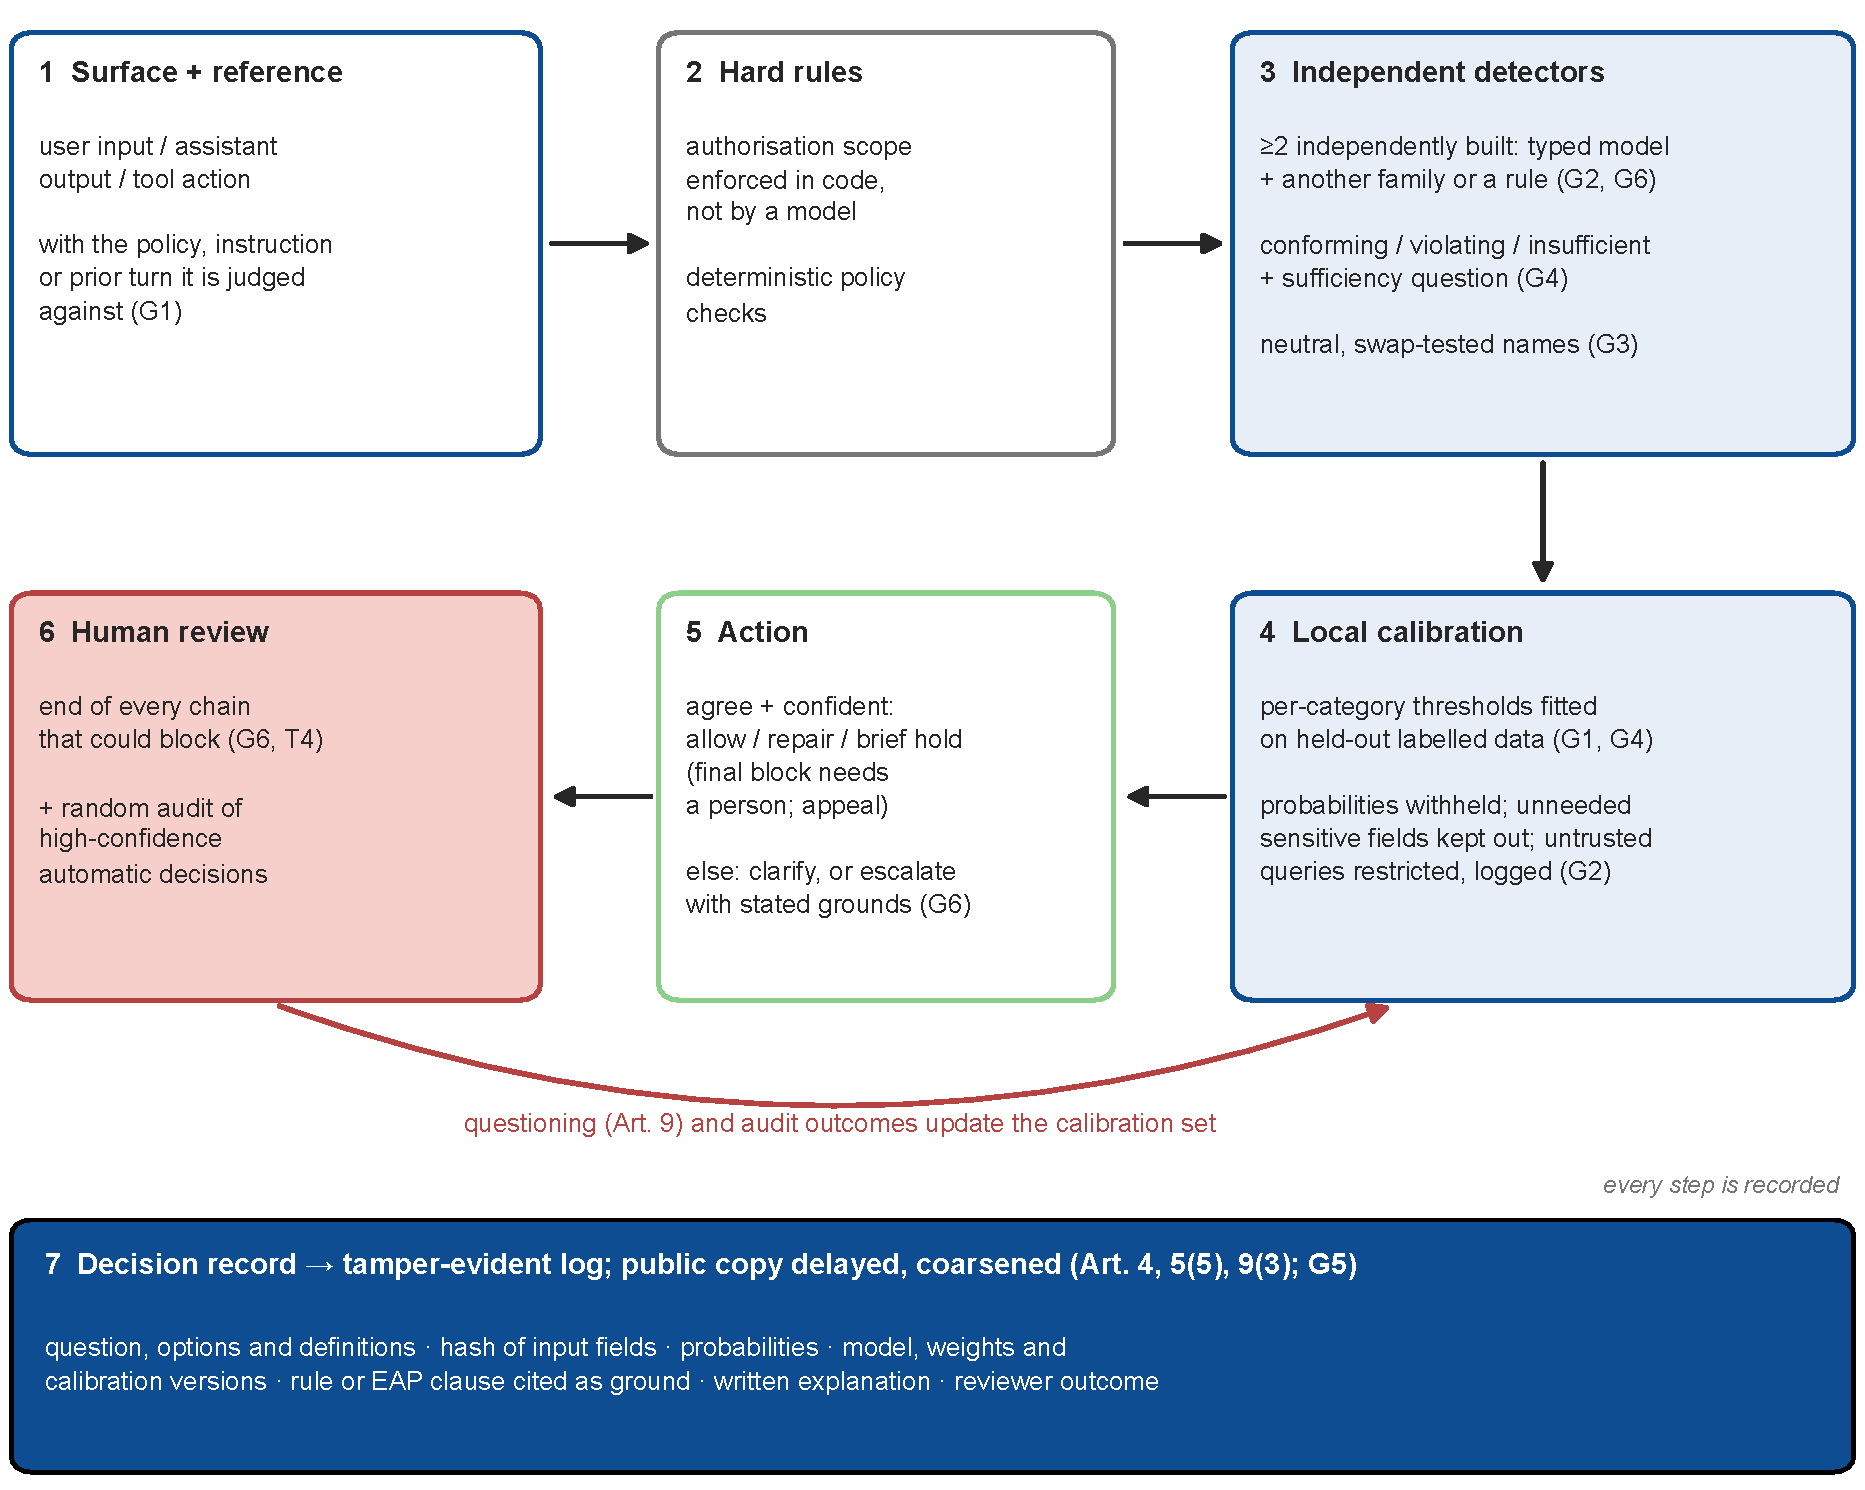
\includegraphics[width=0.8\linewidth]{figures/fig_architecture.pdf}
\caption{A reference design for a clause-governed safety valve. Typed models are detectors (3) whose output is calibrated locally (4) before any automatic action (5); disagreements and insufficient information are clarified or escalated, any final block is confirmed by a person, and a random sample of confident automatic decisions is audited by people (6); every step is written to a decision record (7). Labels in parentheses give the requirement or tension that motivates each element.}
\label{fig:architecture}
\end{figure}

\begin{enumerate}
  \item \textbf{Give the detector the reference, not only the text}, and compute facts that require arithmetic or inference in code or in a separate logged step~\cite{arx29429,arx39496,arx01834}.
  \item \textbf{Enforce scope in code}, by capability checks before any model is consulted~\cite{arx22664}.
  \item \textbf{Use at least two independently built detectors}, ask three-valued questions with sufficiency asked separately, bind neutral option identifiers to definitions and test them by renaming, and ask flags that must fail independently in separate calls~\cite{arx29769,arx02048,arx01006,arx26758,zen23038928}.
  \item \textbf{Calibrate locally and re-certify} per category, for every new question type and over time. Keep raw probabilities from untrusted callers, keep fields a decision does not need out of the detector's input, and restrict and log untrusted queries~\cite{arx24052,arx33689,arx30243,arx04985}.
  \item \textbf{Act automatically only on agreement, and restrict people only briefly and reversibly}. Agreement plus calibrated confidence allows an automatic \emph{allow}, automatic \emph{repair} of the AI system's own output (never the editing of a person's message), and a \emph{hold} of a person's content that is limited in time and fully reversible. A final block of speech, a benefit or an account requires confirmation by a person and remains open to appeal.
  \item \textbf{End every chain that could block with a person, and audit confident decisions} by random sample, with the model's verdict hidden from the auditor~\cite{arx29769,arx33401,parasuraman2010complacency}.
  \item \textbf{Record every decision} in a tamper-evident log whose public version is delayed and coarsened. It holds the question, options and definitions, an input hash, the probabilities, the model and calibration versions, the ground cited and the reviewer's outcome.
\end{enumerate}
Element~5 keeps the typed model a detector.
The design has costs. Requiring agreement lowers sensitivity, risk-control guarantees do not hold under adaptive attack, and separate calls and a second detector multiply cost and latency.
Most elements rest on evidence of low or very low certainty, so the design is a hypothesis to be tested on the \pol{} construct and has not been validated.
\oa{D} turns the evidence into 16 acceptance tests with provisional pass criteria for any model proposed for such a safeguard.

\subsection{Verdict: is hosted Jev a suitable governance tool for \pol{}?}
\label{sec:verdict}

\Cref{tab:verdict-summary} gives a verdict for each \pol{} function that a typed model could be asked to perform.
\oa{D} gives the deciding evidence for each verdict and what would be needed to change it.
The verdicts concern hosted \jev{} at its versions of 15~September to 8~October 2026 and, where a finding's scope is ``both'', typed models generally.
They are not predictions about later models.

\begin{table}[t]
\centering
\footnotesize
\caption{Verdict for \pol{}, function by function (full table with the deciding evidence: \oa{D}). NS, not supported; DC, supported only as a recorded detector with conditions (the design of \cref{sec:design}); NT, not tested on \pol{}'s construct. Certainty is the rating of the deciding findings in \cref{tab:keyfindings}; $^{c}$~contested; ``not rated'' marks single-study results that are not key findings.}
\label{tab:verdict-summary}
\begin{tabularx}{\linewidth}{@{}>{\raggedright\arraybackslash}p{0.26\linewidth}>{\raggedright\arraybackslash}p{0.09\linewidth}L>{\raggedright\arraybackslash}p{0.17\linewidth}@{}}
\toprule
\pol{} function & Req. & Verdict & Certainty \\
\midrule
Safety valve: blocking hate language in inputs (\clause{5.4.1}) & G1--G3, G6 & DC: automatic \emph{hold} only on agreement of independently built detectors; final block by a person & low; low$^{c}$ (thresholds) \\
Truncation of PAI's own output (\clause{4.3.3.1}) & G1, G3, G5 & DC: automatic \emph{repair} of the AI's own output, with a record of what was removed & low \\
Real-time correction support (\clause{4.3.3.2}) & G1, G5 & NT: the typed interface covers identification only; suggestions untested & low; not rated \\
Anomaly detection and risk warning (\art{7}(2)--(3)) & G1, G2, G6 & DC on text; NS on numeric or structured signals without a trained model & low; very low \\
Automatic ethical verification (\art{6}(3)) & G3--G5 & NS as an automatic verifier; the EAP construct NT & very low; low \\
Dispute adjudication without human intervention (\art{10}, \art{9}(7)) & G4--G6 & NS as judge; DC only for ranking and triage of filings & low; low$^{c}$ (thresholds) \\
Per-person quantification (\clause{5.6}) & G3, G7 & NS as a decision input; NT on error by group, so score events, not persons (precautionary) & very low; low; not rated \\
Assessment dimension in public decisions (\clause{5.6}) & G7 & DC: an audited aggregate measurement with its measured error carried into every conclusion; not a decision input on its own & very low; not rated \\
\bottomrule
\end{tabularx}
\end{table}

\paragraph{The verdict.}
On the evidence to 8~October 2026, hosted \jev{} is not a suitable tool for any \pol{} function that decides: dispute adjudication under \art{10}, automatic ethical verification under \art{6}(3), the per-person quantification of \clause{5.6} (on steering and, since no study measures error by group, on precaution), and any use of the safety valve in which a block of a person's speech is final without a person's confirmation.
The decisive findings are negative and, within their low or very low certainty, consistent.
Thresholds fitted in one setting do not transfer (low, contested), content inside what the model audits can steer its decisions (low), and option names can override their definitions (low).
An explicit ``I don't know'' option is rarely chosen when it is correct, and ``none'' inconsistently (low).
The low-cost evaluators to which such a model would escalate repeated almost all of its confident errors (low, an upper bound).
A judge with these properties would restrict speech and allocate welfare on verdicts that an adversary can move and that no second automated opinion is likely to catch.
By keeping human supervision from intervening, \art{9}(7) would remove the one check the evidence says is needed.
Where the comparison was made, typed models were not generally worse (low, by judgement).
Most failures, however, were never compared with generative evaluators, so the verdict is not specific to typed models.
Until such evaluators are tested under the same protocol, it applies as a precaution to automated judges of this cost tier.

For the functions that detect (the safety valve, truncation of PAI's own output and anomaly detection on text), hosted \jev{} is usable only inside the design of \cref{sec:design}, and the public-decision assessment of \clause{5.6} only as an audited aggregate measurement.
Even this extrapolates from English benchmarks of binary hate speech.
No study measures \pol{}'s three-valued construct in Chinese, and the only Chinese emotion result found every system weak~\cite{arx08829}.
Every system tested separated hate from merely offensive language only weakly, and this is the distinction \clause{1.5} most needs~\cite{arx03324}.
Two further findings bear on \pol{} as a whole.
First, with conditional instructions planted in the input, hosted \jev{}'s labels alone revealed hidden attributes (an open model's revealed none).
A typed safeguard can therefore serve as a queryable oracle, and the protective measures of element~4 have not been tested against this~\cite{arx04985}.
Second, a closed hosted model cannot satisfy \art{4} and \art{5}(4) as written (T3).

\paragraph{What transfers.}
Whatever model is used, the evidence supports practices tied to the interface and the task rather than to \jev{}.
On this evidence, questions should be three-valued, with sufficiency asked separately, neutral identifiers bound to definitions and tested by renaming, and every decision recorded.
Calibration should be local and periodically re-validated, since for 20 language models in English (no typed model tested) hate-speech rankings on static benchmarks did not predict rankings on time-stamped data~\cite{dibonaventura2025hatevolution}.
Automatic action should require agreement between differently built detectors, and chains that could restrict a person should end with a person, with blind audit of confident decisions.
Probabilities should be withheld from untrusted callers, and sensitive fields that a decision does not need should be kept out of the input.
Scores should attach to events and behaviours, never to persons.
Measuring these practices on \pol{}'s construct, rather than extrapolating from English, requires a construct benchmark in Chinese.
Several of these are already \pol{}'s own commitments: the state of absence, the warning that love and hate are not moral labels, and the distinction between persons and behaviours.
